
%%
%% This is file `sample-sigconf.tex',
%% generated with the docstrip utility.
%%
%% The original source files were:
%%
%% samples.dtx  (with options: `sigconf')
%% 
%% IMPORTANT NOTICE:
%% 
%% For the copyright see the source file.
%% 
%% Any modified versions of this file must be renamed
%% with new filenames distinct from sample-sigconf.tex.
%% 
%% For distribution of the original source see the terms
%% for copying and modification in the file samples.dtx.
%% 
%% This generated file may be distributed as long as the
%% original source files, as listed above, are part of the
%% same distribution. (The sources need not necessarily be
%% in the same archive or directory.)
%%
%% The first command in your LaTeX source must be the \documentclass command.
\documentclass[sigconf]{acmart}
\graphicspath{ {./imgs/} }
%%
%% \BibTeX command to typeset BibTeX logo in the docs
\AtBeginDocument{%
  \providecommand\BibTeX{{%
    \normalfont B\kern-0.5em{\scshape i\kern-0.25em b}\kern-0.8em\TeX}}}

%% Rights management information.  This information is sent to you
%% when you complete the rights form.  These commands have SAMPLE
%% values in them; it is your responsibility as an author to replace
%% the commands and values with those provided to you when you
%% complete the rights form.
%%\setcopyright{acmcopyright}
%%\copyrightyear{2018}
%%\acmYear{2018}
%%\acmDOI{10.1145/1122445.1122456}

%% These commands are for a PROCEEDINGS abstract or paper.
%%\acmConference[Woodstock '18]{Woodstock '18: ACM Symposium on Neural
%%  Gaze Detection}{June 03--05, 2018}{Woodstock, NY}
%%\acmBooktitle{Woodstock '18: ACM Symposium on Neural Gaze Detection,
%%  June 03--05, 2018, Woodstock, NY}
%%\acmPrice{15.00}
%%\acmISBN{978-1-4503-XXXX-X/18/06}


%%
%% Submission ID.
%% Use this when submitting an article to a sponsored event. You'll
%% receive a unique submission ID from the organizers
%% of the event, and this ID should be used as the parameter to this command.
%%\acmSubmissionID{123-A56-BU3}

%%
%% The majority of ACM publications use numbered citations and
%% references.  The command \citestyle{authoryear} switches to the
%% "author year" style.
%%
%% If you are preparing content for an event
%% sponsored by ACM SIGGRAPH, you must use the "author year" style of
%% citations and references.
%% Uncommenting
%% the next command will enable that style.
%%\citestyle{acmauthoryear}

%%
%% end of the preamble, start of the body of the document source.
\begin{document}

%%
%% The "title" command has an optional parameter,
%% allowing the author to define a "short title" to be used in page headers.
\title{Vulnerabilities in WebAssembly: A Survey}

%%
%% The "author" command and its associated commands are used to define
%% the authors and their affiliations.
%% Of note is the shared affiliation of the first two authors, and the
%% "authornote" and "authornotemark" commands
%% used to denote shared contribution to the research.
\author{Holger Klein}
%%\authornote{Both authors contributed equally to this research.}
%%\email{uaidx@student.kit.edu}
%%\orcid{1234-5678-9012}
%%\author{G.K.M. Tobin}
%%\authornotemark[1]
%%\email{webmaster@marysville-ohio.com}
\affiliation{%
  \institution{Karlsruhe Institute of Technology (KIT)}
%%  \streetaddress{P.O. Box 1212}
  \city{Karlsruhe}
%%  \state{Deutschland}
  \country{Germany}
%%  \postcode{43017-6221}
}


%%
%% By default, the full list of authors will be used in the page
%% headers. Often, this list is too long, and will overlap
%% other information printed in the page headers. This command allows
%% the author to define a more concise list
%% of authors' names for this purpose.
\renewcommand{\shortauthors}{Holger Klein}

%%
%% The abstract is a short summary of the work to be presented in the
%% article.
\begin{abstract}
  A clear and well-documented \LaTeX\ document is presented as an
  article formatted for publication by ACM in a conference proceedings
  or journal publication. Based on the ``acmart'' document class, this
  article presents and explains many of the common variations, as well
  as many of the formatting elements an author may use in the
  preparation of the documentation of their work.
\end{abstract}

%%
%% The code below is generated by the tool at http://dl.acm.org/ccs.cfm.
%% Please copy and paste the code instead of the example below.
%%

%%
%% Keywords. The author(s) should pick words that accurately describe
%% the work being presented. Separate the keywords with commas.
\keywords{binary exploits, Webassembly, IT Security}

%% A "teaser" image appears between the author and affiliation
%% information and the body of the document, and typically spans the
%% page.
\begin{teaserfigure}
  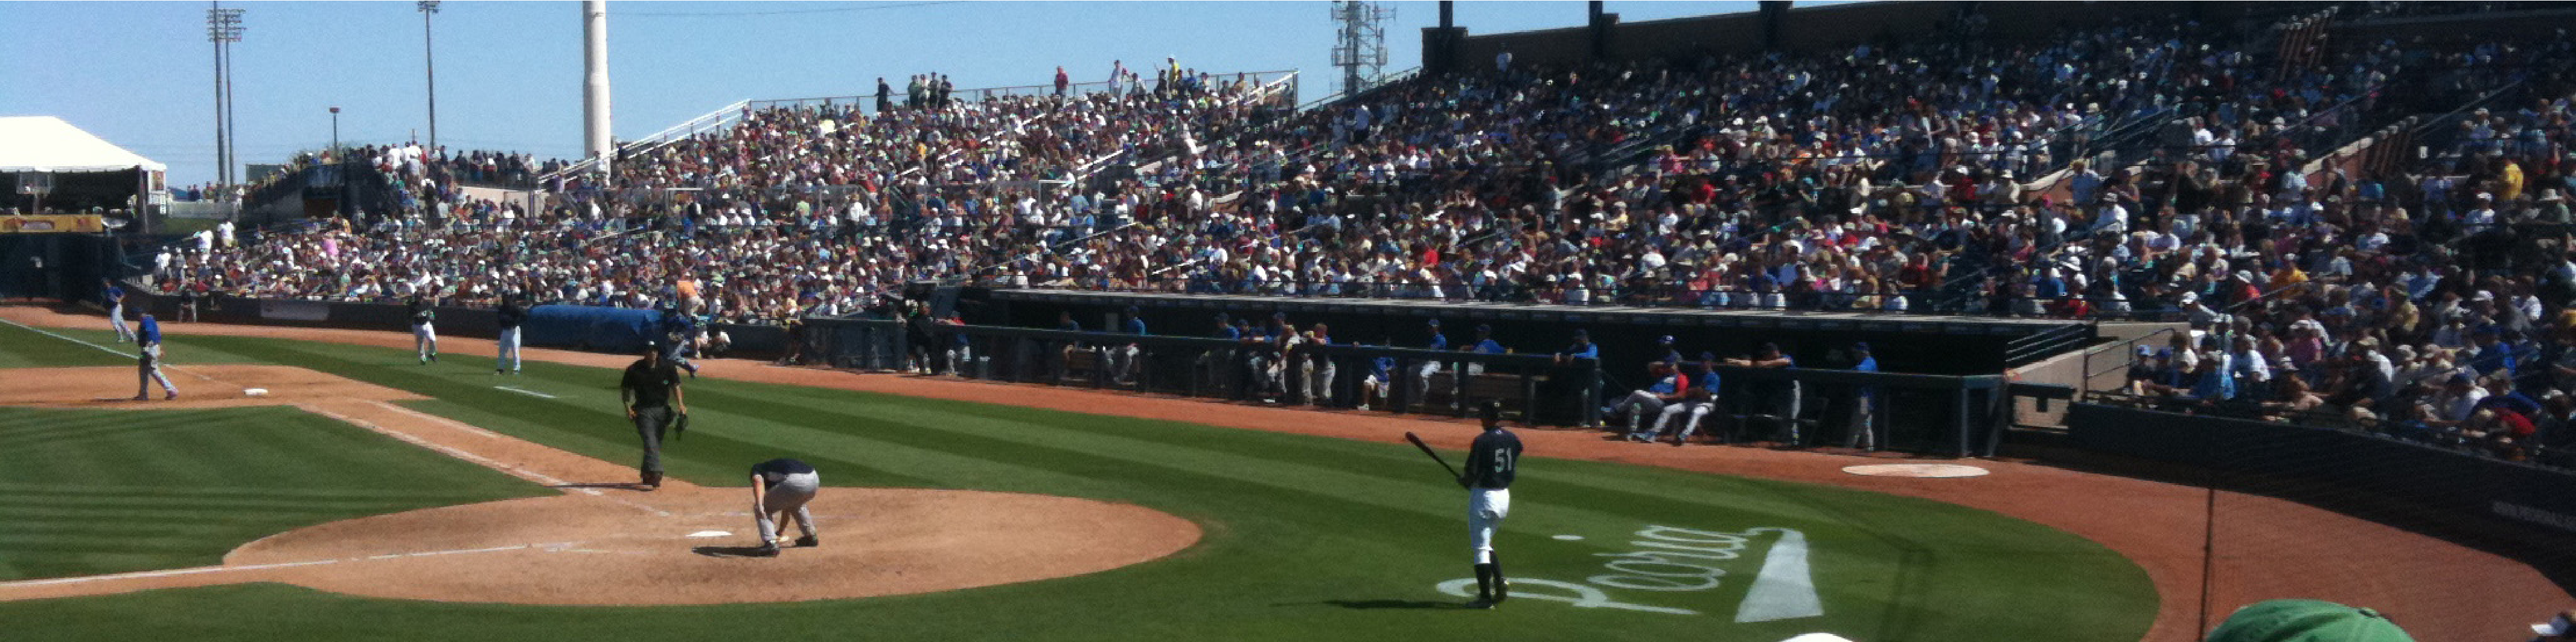
\includegraphics[width=\textwidth]{sampleteaser}
  \caption{Seattle Mariners at Spring Training, 2010.}
  \Description{Enjoying the baseball game from the third-base
  seats. Ichiro Suzuki preparing to bat.}
  \label{fig:teaser}
\end{teaserfigure}

%%
%% This command processes the author and affiliation and title
%% information and builds the first part of the formatted document.
\maketitle

\section{Introduction}
WebAssembly is a binary code format and compilation target meant to bring performance to web applications.  The initial design of the API and binary format of WebAssembly got completed in 2017 \cite{wasm_roadmap}. Since then, most major browsers such as Firefox, Chrome or Safari implement many of the proposed features. Even in the backend it is possible to run code compiled to WebAssembly for example when using Nodejs. The promise of running code with near native performance in the browser is very attractive, as it allows for more demanding web applications and smoother user experiences. However, since any Website visited by the user can download and execute WebAssembly code just like Javascript, it immediately raises security concerns. On the one hand, a malicious website could execute malware on the host PC or use computing ressources by executing a crypto miner. On the other hand, a vulnerable WebAssembly program which takes user input could lead to cross site scripting attacks in the browser. Worse yet, as WebAssebly gets adopted in the backend or even in stand-alone applications, vulnerabilities in WebAssembly programs could enable attacks such as Remote Code Execution. This survey will mainly deal with issues of the latter kind, focusing on how WebAssembly programs might be vulnerable to binary exploits. In particular, we will focus on how the security mechanisms intrinsic to WebAssembly's design compare to binary exploit mitigations in native applications. 
The official spec adresses some of the security concerns by stating that "[...] code is validated and executes in a memory-safe*, sandboxed environment preventing data corruption or security breaches". However, it adds a footnote which specifies "*No program can break WebAssembly’s memory model. Of course, it cannot guarantee that an unsafe language compiling to WebAssembly does not corrupt its own memory layout, e.g. inside WebAssembly’s linear memory". Indeed, in the past years there have been a few puplications commenting on WebAssembly's lack of mitigations to common binary exploitation techniques, such as \cite{mcfadden_security_2018} or \cite{lehmann_everything_2020}. Additionally, there have been puplications researching the real-world assembly programs such as \cite{musch_new_2019} or \cite{hilbig_empirical_2021}. In this survey, we aim to cover the main points of these publications and try to recreate their main results. It is structured as follows: \ref{sec:wasm} will introduce WebAssembly with a focus on the features which will be important to our discussion later. ASDASDASDASD

\section{WebAssembly}
\label{sec:wasm}
The following will give an Introduction to and and overview of WebAssembly, paying special attention to the parts relevant to a discussion of binary vulnerabilities. For more information, see the official specification at \cite{webAssembly_spec_2021}, or the Background section in \cite{lehmann_everything_2020}. 

\subsection{High Level Overview}
The name 'WebAssembly' (often abbreviated as WASM) is a slight misnomer, since it has a different form and function from typical assembly languages. The official spec refers to it as "low-level, assembly-like". It is a binary byte code format which is interpreted by a Virtual Machine, similar to for example Java. The Virtual Machine is most often implemented in a browser. Design goals were to make WebAssembly safe, hardware- and language independent and fast. In fact, WebAssembly is supposed to run at near-native speeds. There exists a human-readable format of WebAssembly binaries called 'wat'. Whenever we present WebAssembly Code, it will be in this format. While it is possible to hand-craft wasm binary, it is most often generated by compiling a high-level language such as C/C++ or Rust. The Binary is then instantiated by calling a Javascript function. See \ref{fig:wasm_init_firefox}. By itself, a compiled WebAssembly module has now way of communicating with the host environment such as a Browser (assuming a Bug-free Virtual Machine). WebAssembly functionality can only be accessed by calling functions which are exported by the WebAssembly module. These exported functions can be called from Javascript code. Conversely, WebAssembly has no I/O other than what is directly supplied through imported Javascript functions. 

\begin{figure}[h]
  \centering
  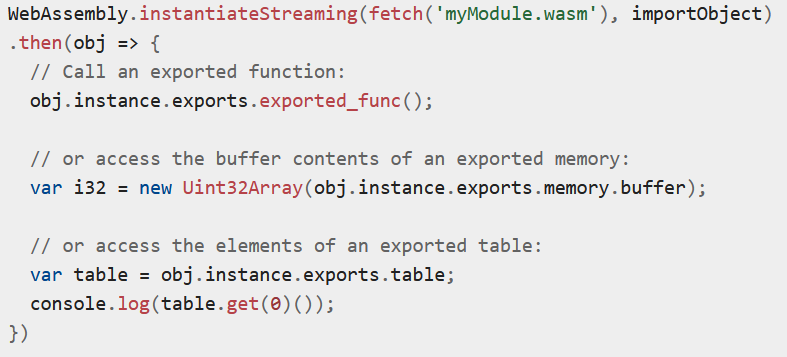
\includegraphics[width=0.5\textwidth]{wasm_init_firefox}
  \caption{How to intantiate a WebAssembly module using Javascript. (\url{https://developer.mozilla.org/en-US/docs/WebAssembly/Loading_and_running}).}
\end{figure}


\subsection{Modules}
At the highest level, WebAssembly programs are organized into Modules.  A module is what gets compiled and run by the Virtual Machine. Amongst other things, a module contains definitions for imports and exports, functions, types, tables and memories. All definitions are referenced by zero-based indices. As of the time of writing, only one memory may be defined in a module. This memory is indexed by 0 and implicitely referenced by all other constructs. More on memory in \ref{sec:memories}. Also as of time of writing the only table elements which are available are untyped function references. This is used to implement indirect function calls, see \ref{sec:indirect_calls}. For an example of WebAssembly code, see 

\begin{figure}[h]
  \centering
  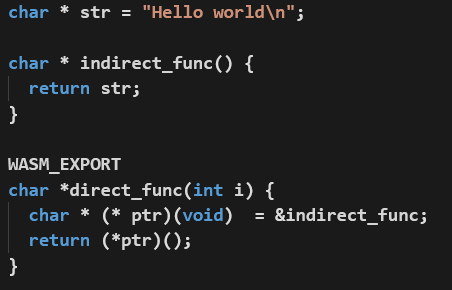
\includegraphics[width=0.5\textwidth]{wasm_example_c}
  \caption{A c program, which, when compiled without optimization, gets translated to the code in Figure  \ref{fig:wasm_example_wasm}.}
\label{fig:wasm_example_c}
\end{figure}

\begin{figure}[h]
  \centering
  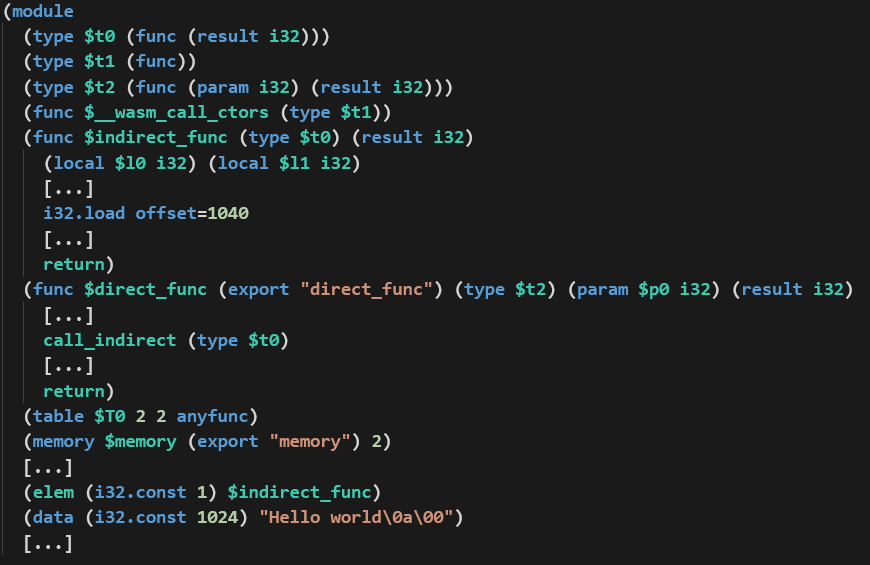
\includegraphics[width=0.5\textwidth]{wasm_example_wasm}
  \caption{The c program in Figure \ref{fig:wasm_example_c} gets compiled to this WebAssembly program (with uninteresting parts removed). Observe the function table and memory.}  
\label{fig:wasm_example_wasm}
\end{figure}

\subsection{The Stack}
\label{sec:wasm_stack}
The WebAssembly virtual machine is Stack based. Thus, it doesn't have registers. Instead, values are pushed on and popped of the stack. All instructions implicitely operate on the stack. 

\subsection{Control Flow}
\label{sec:wasm_control_flow}
In contrast to native languages or even Java, WebAssembly enforces structured control flow. Code can only be organized into blocks. Control-flow commands can only jump to the beginning of such a block, and only within the current function. In addition, the bytecode never interacts with the underlying adresses of functions. These are only accesible to the Virtual Machine. This immediately makes many binary exploits infeasable, such as Return-Oriented Programming. 

\subsection{Memories} 
\label{sec:memories}
WebAssembly only supports four different primitive types: 32- and 64-bit Integers (i32, i64) and single- and double-precision floating point nubmers (f32, f64). As such, arrays, pointers, etc. have no explicit representation at the binary level. To see how they are implemented in binary programs, it is necessary to understand the way WebAssembly handles memory. The implementation of function pointers is discussed in \ref{sec:indirect_calls}. The Stack of a function which contains the return adress as well as any native data type whose adress is never taken is not accesible to the bytecode. As mentioned in \ref{sec:wasm_control_flow}, this in itself contributes to WebAssemblys inherent security. However, anything other than a value of native type or any value whose adress is taken needs to reside in the linear memory. This memory is a linear array of bytes. Adresses are referenced by 32 bit integers which serve as pointer types.   The WebAssembly program can request more memory from the Host VM using the memory.grow operation. The linear memory is completely unmanaged. The way it is used is completely up to the program. Many WebAssembly toolchains such as Emscripten include an allocator which implements functions such as C's malloc and free. This unmanaged, linear memory is the main vector of attack of all vulnerabilities discussed in \cite{lehmann_everything_2020}. As will be discussed in section  \ref{sec:binary_vulns}.


\subsection{Indirect Function Calls} 
\label{sec:indirect_calls}
To implement indirect function calls, any function which may get called indirectly or used as a function pointer has an entry in the table section. The \textbf{call\_indirect}  operation pops an index from the stack which is used to reference an entry in the table section. This table maps the index to a function. This limits which functions can be called indirectly. Additionally, functions in WebAssembly are type checked. The \textbf{call\_indirect} operation has the function type statically encoded. Thus, an indirect call can only call functions which have the same signature. It must be remarked however that this is less limiting than it might first appear, since WebAssembly only has four native types. Thus, a function taking a pointer (or a string) has the same signature as a function taking an 32-bit Integer.

\subsection{Deployment, Compilers and Toolchains}
It would be very impractical (albeit possible) to write WebAssembly from scratch. Thus, several Backends exist to generate WebAssembly bytecode from high-level languages such as C, Go or Rust. Emscripten \cite{emscripten} can not only generate the Bytecode from C/C++ but also html and Javascript to load and run the WebAssembly module. It also comes with C Headers to interact with the Browser and implements several common libraries such as SDL2 \cite{sdl2}.  

\section{Binary Vulnerabilities of WebAssembly programs}
\label{sec:binary_vulns}
In this section we will discuss the security vulnerabilities of WebAssembly as presented in \cite{mcfadden_security_2018} and \cite{lehmann_everything_2020}. \cite{lehmann_everything_2020} begin by discussing the security related aspects of the linear unmanaged memory. As mentioned in \ref{sec:memories}, every scalar value whose adress is never taken, as well as function return adresses are completely controlled by the virtual machine. This mitigates many well-known attacks. However, all non-scalar types such as arrays or any value whose adress is ever taken must lie in the unmanaged memory. This memory is usually controlled by an allocator provided by the compilation toolchain. Most allocators seperate the memory in three distinct regions: The Stack, Heap and Data sections. To distinguish between the function call stack managed by the VM and the call stack created by the compiler, \cite{lehmann_everything_2020} call the latter the \textbf{unmanaged} stack. We will use the same nomenclature here. One must keep in mind however, that there are no underlying mechanisms provided by the VM to seperate between these three regions. This seperation is only implemented by the compiler. Initially, it is just a single contiguous linear array of bytes. 

\subsection{Exploitation potential of unmanaged memory}
\cite{mcfadden_security_2018} discuss serveral common exploit mitigation techniques which are used in binary programs. Table \ref{table:exploit_mitigation_wasm} provides a summary and shows whether these techniques are present in WebAssembly.

\begin{table*}
\begin{tabular}{p{2cm} | p{2cm} | p{6cm} | p{6cm} }
  \toprule
  Exploit mitigation & Protect against & Effect in Native Binaries & WebAssembly \\
  \midrule
  Address Space Layout Randomization (ASLR) & Attacks on Control-Flow & Randomizes the base adress of an executable as well as the heap and stack adresses and adresses of libraries. This is meant to make exploitation techniques such as Return Oriented Programming harder. It also makes exploiting other vulnerabilities more challenging& ASLR has no equivalent mechanism in WebAssembly. However, since the user can't access Return Adresses, many exploits that rely on changing control flow are infeasible. In addition, since WebAssembly only provides 32-bit adresses, it is assumed to have to little entropy for ASLR to be effective. Also, since functions are directly accessed by indices instead of memory adresses, ASLR could not be used to obfuscate function adresses. \\ \hline
   Stack Canaries & Stack-based Buffer overflows & Stack Canaries are placed on the stack such that a stack-based buffer overflow will overwrite them before corrupting the functions return adress. This enables the program to detect and handle these overflows & Stack canaries don't exist in WebAssembly, since the return adresses are entirely managed by the VM \\ \hline
   Heap Hardening & Manipulating Allocator Metadata & Heap Hardening comprises several different programming techniques to make Allocators more secure against attacks. By corrupting heap metadata, an attacker can use the allocator to execute arbitrary writes on the heap. & Since size is a concern, many toolchains deploy with their own smaller allocator which might have vulnerabilities.\\ \hline
   Data Execution Prevention (DEP) & Code injection & This mitigation is part of a family of mitigations which modify memory pages to only allow certain behaviour. These can modify whether the contents of certain memory pages can be executed. In native binaries, this can prevent the injection of malicious code & In webassembly, there is a strict seperation between code and data. Hence, DEP is not needed. \\ \hline
   
\label{table:exploit_mitigation_wasm}
\end{tabular}
\end{table*}

\cite{lehmann_everything_2020} similary discuss common mitigations such as ASLR and page protection flags which are not present in WebAssembly. In particular, since there are no guard pages between the different sections of the linear memory , an overflow in any section can corrupt data in any other section. And since there is no concept of read-only memory, even data which is marked as constant in the source code can be overwritten during execution.  

\section{Attacking Vulnerabilities}
Having analyzed WebAssemblys main vulnerability, the unmanaged linear memory, there are several ways to exploit these.  \cite{mcfadden_security_2018} show two attack primitives, format-string attacks and stack-based buffer overflows. They use these attack primitives to implement a proof of concept of a cross-site scripting attack, and remote code execution on a server.  \cite{lehmann_everything_2020} similarly first demonstrate two write primitves. They first introduce a stack-based buffer overlfow. They also demonstrate how the allocators supplied by emscripten are succeptible to the so-called unlink exploit. This can be utilized to allow an attacker to write an arbitrary value to an arbitrary adress. However, we couldn't recreate their exploit using the current version of emscripten. Nevertheless, we will quickly summarize the presented attack primitives. Afterwards we will demonstrate our attempt to recreate these attack primitives.

\subsection{format string attacks}

\subsection{Stack Based buffer overflows}

\subsection{Heap Metadata corruption}

\bibliographystyle{ACM-Reference-Format}
\bibliography{Wasm-Vuln}

%%
%% If your work has an appendix, this is the place to put it.
\appendix


\end{document}
\endinput
%%
%% End of file `sample-sigconf.tex'.'